\chapter{How to Cheat}
\label{ch:how_to_cheat}

\begin{wrapfigure}{o}{0.85\textwidth}
    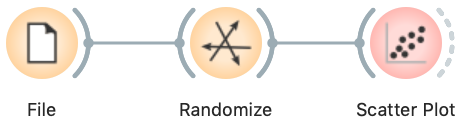
\includegraphics[scale=0.4]{workflow-randomize.png}
\end{wrapfigure}

At this stage, \marginnote[-2cm]{This lesson has a strange title and it is not obvious why it was chosen. Maybe you, the reader, should tell us what this lesson has to do with cheating.} the classification tree looks very good. There’s only one data point where it makes a mistake. Can we mess up the data set so bad that the trees will ultimately fail? Like, remove any existing correlation between features and the class? We can! There's the \widget{Randomize} widget with class shuffling. Check out the chaos it creates in the \widget{Scatter Plot} visualization where there were nice clusters before randomization!

\begin{figure*}[h]
    \infinitewidthbox{
    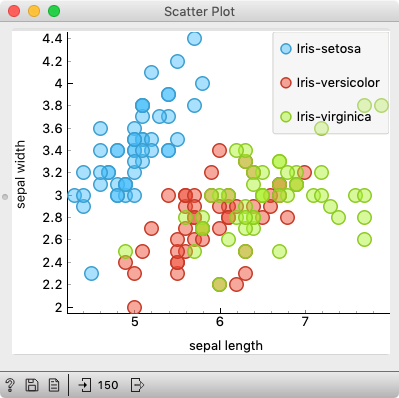
\includegraphics[scale=0.4]{scatterplot_iris.png}
    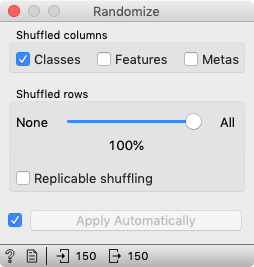
\includegraphics[scale=0.4]{randomize100.png}
    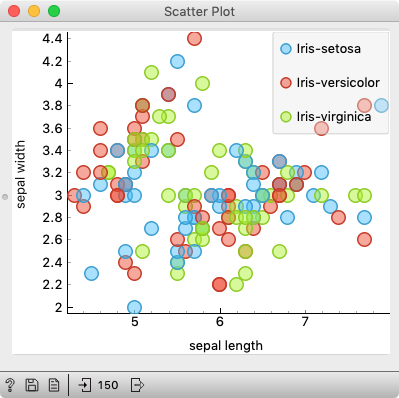
\includegraphics[scale=0.4]{scatterplot_iris_random.png}
    }
    \caption{Left: scatter plot of the \textit{Iris} data set before randomization; right: scatter plot after shuffling 100\% of rows.}
\end{figure*}

Fine. There can be no classifier that can model this mess, right? Let’s make sure.

\begin{figure}[h]
    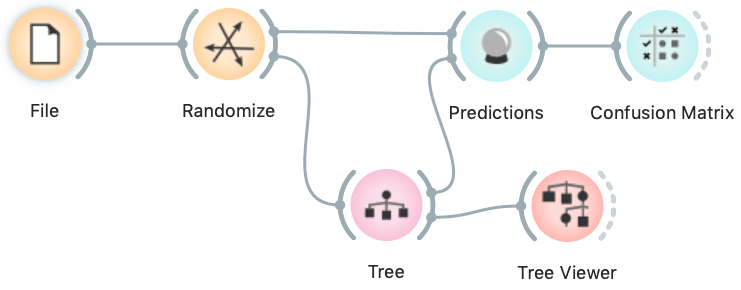
\includegraphics[scale=0.4]{workflow_classification.png}
    \caption{$\;$} % empty caption for correct alignment
\end{figure}

\begin{wrapfigure}{o}{0.85\textwidth}
    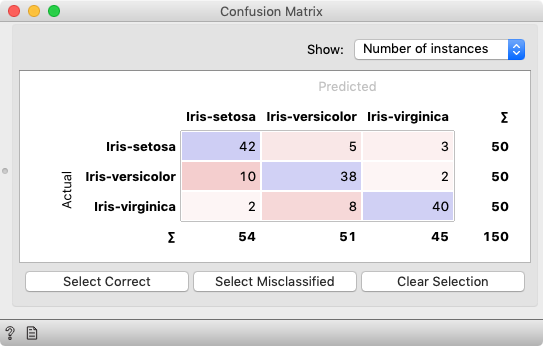
\includegraphics[scale=0.35]{confusion_randomized.png}
\end{wrapfigure}

And the result? Here is a screenshot of the \widget{Confusion Matrix}.

Most unusual. Despite shuffling all the classes, which destroyed any connection between features and the class variable, about 80\% of predictions were still correct.

\clearpage

Can we further improve accuracy on the shuffled data? Let us try to change some properties of the induced trees: in the \widget{Tree} widget, disable all early stopping criteria.

\begin{figure}[h]
    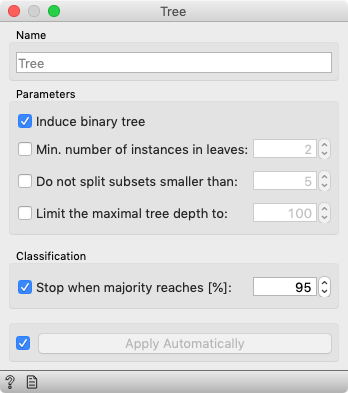
\includegraphics[scale=0.35]{better_tree.png}
    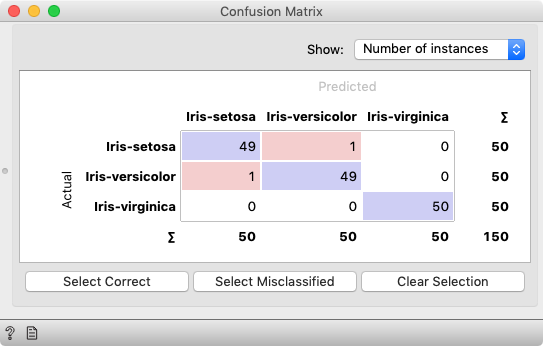
\includegraphics[scale=0.35]{confusion_randomized_better.png}
    \caption{After we disable 2--4 check box in the \widget{Tree} widget, our classifier starts behaving almost perfectly.}
\end{figure}


Wow, almost no mistakes now. How is this possible? On a class-randomized data set?

\begin{wrapfigure}{o}{0.85\textwidth}
    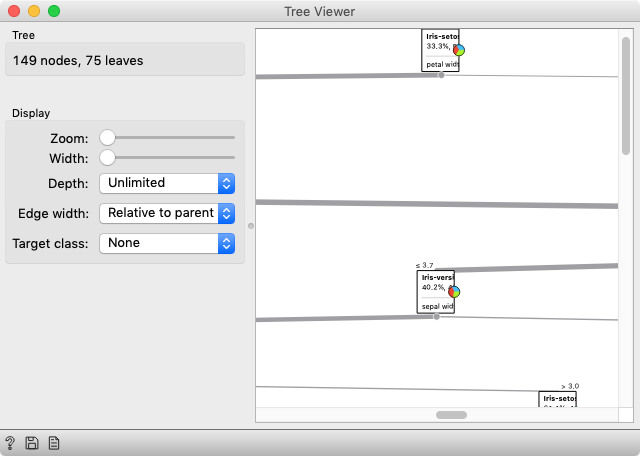
\includegraphics[scale=0.4]{tree_viewer.png}
    \caption{In the build tree, there are 75 leaves. Remember, there are only 150 rows in the \textit{Iris} data set.}
\end{wrapfigure}

To find the answer to this riddle, open the \widget{Tree Viewer} and check out the tree. How many nodes does it have? Are there many data instances in the leaf nodes?

Looks like the tree just memorized every data instance from the data set. No wonder the predictions were right. The tree makes no sense, and it is complex because it simply remembered everything.

Ha, if this is so, if a classifier remembers everything from a data set but without discovering any general patterns, it should perform miserably on any new data set. Let us check this out. We will split our data set into two sets, training and testing, train the classification tree on the training data set and then estimate its accuracy on the test data set.

\begin{figure}[h]
    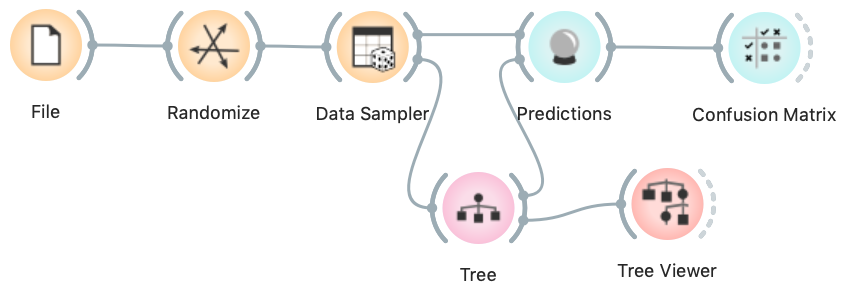
\includegraphics[scale=0.35]{workflow_data_sampler.png}
    \caption{Connect the \widget{Data Sampler} widget carefully. The \widget{Data Sampler} splits the data to a sample and out-of-sample (so called remaining data). The sample was given to the \widget{Tree} widget, while the remaining data was handed to the \widget{Predictions} widget. Set the \widget{Data Sampler} so that the size of these two data sets is about equal.}
\end{figure}

Let’s check how the \widget{Confusion Matrix} looks after testing the classifier on the test data.

The first two classes are a complete fail. The predictions for ribosomal genes are a bit better, but still with lots of mistakes. On the class-randomized training data our classifier fails miserably. Finally, just as we would expect.

\begin{figure}[h]
    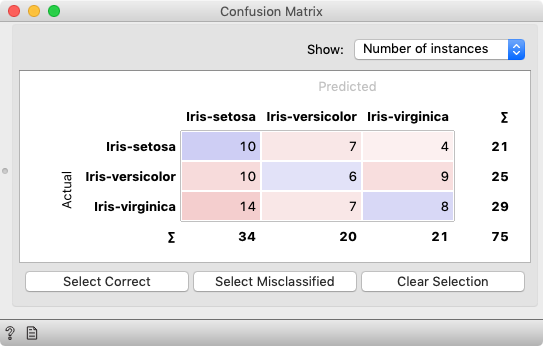
\includegraphics[scale=0.4]{confusion_sampler.png}
    \caption{Confusion matrix if we estimate accuracy on a data set that was not used in learning.}
\end{figure}

We have just learned that we need to train the classifiers on the training set and then test it on a separate test set to really measure performance of a classification technique. With this test, we can distinguish between those classifiers that just memorize the training data and those that actually learn a general model.

Learning is not only memorizing. Rather, it is discovering patterns that govern the data and apply to new data as well. To estimate the accuracy of a classifier, we therefore need a separate test set. This estimate should not depend on just one division of the input data set to training and test set (here's a place for cheating as well). Instead, we need to repeat the process of estimation several times, each time on a different train/test set and report on the average score.